\documentclass{article}
\usepackage[utf8]{inputenc}
\usepackage{graphicx}

\begin{document}

\section{10 Q4}

Sellers a, b, and c are selling their houses for prices of 3, 1, and 0, respectively.\\\\
Buyer x values house a at 12, house b at 9, and house c at 8.\\
Buyer y values house a at 10, house b at 3, and house c at 6.\\
Buyer z values house a at 8, house b at 6, and house c at 5.\\
\\
Buyer x receives the maximum payoff by purchasing from Seller a.\\
\indent Payoff with a  = 12 - 3 = 9.\\\\
Buyer y receives the maximum payoff by purchasing from Seller a.\\
\indent Payoff with a = 10 - 3 = 7.\\\\
Buyer z receives the maximum payoff by purchasing from either Seller a, b, or c.\\
\indent Payoff with a = 8 - 3 = 5\\
\indent Payoff with b = 6 - 1 = 5\\
\indent Payoff with c = 5 - 0 = 5\\\\

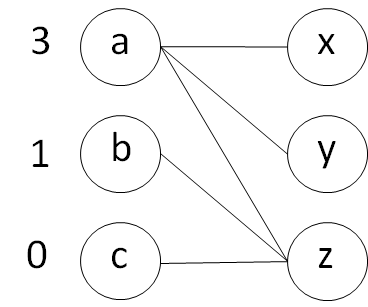
\includegraphics{bipartite_graph1.png}\\\\
This set of prices is not market clearing because Buyers x and y both want to purchase from Seller a in order to maximize their payoffs. Seller a should raise their price in the next round of the bipartite auction procedure.

\section{10 Q5}

Sellers a, b, and c are selling their houses for prices 4, 3, and 1, respectively.\\\\
Buyer x values house a at 7, house b at 7, and house c at 4.\\
Buyer y values house a at 7, house b at 6, and house c at 3.\\
Buyer z values house a at 5, house b at 4, and house c at 3.\\
\\
Buyer x receives the maximum payoff by purchasing from Seller b.\\
\indent Payoff with b  = 7 - 3 = 4.\\\\
Buyer y receives the maximum payoff by purchasing from Sellers a or b.\\
\indent Payoff with a = 7 - 4 = 3.\\
\indent Payoff with b = 6 - 3 = 3.\\\\
Buyer z receives the maximum payoff by purchasing from Seller c.\\
\indent Payoff with c = 3 - 1 = 2\\\\
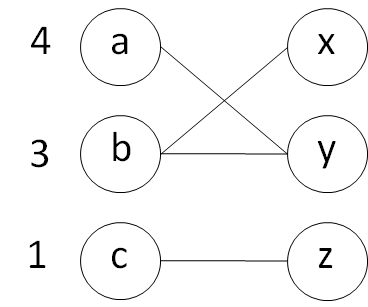
\includegraphics{bipartite_graph2.png}\\\\
This set of prices is market clearing. Buyer x can purchase from Seller b, Buyer y can purchase from Seller a, and Buyer z can purchase from Seller c.  Each buyer purchases from a unique seller and receives their maximum payoff.

\end{document}
